\newpage

\section*{ $^{197}$Au(n,$\gamma$)$^{198}$Au (Cd) }

Power Level: 100 kW(th) \\
Time at Power: 60.0 s \\
Wait Time:  2.0 h \\
Counting Time:  2.0 m \\
Total Activity at Removal: 2.76e+01 $\mu Ci$

\begin{table*}[h]
\centering
\begin{tabular}{ |c|c|c|c|c|c| }
 \hline
 Position & Mass $mg$ & Counting Activity $\mu Ci$ & Area (Counts) & Error \% \\
 \hline 
 1 & 4.10 & 6.10e+00 & 1.22e+06 & 0.0905 \\ 
\hline
 2 & 4.30 & 8.88e+00 & 1.78e+06 & 0.0750 \\ 
\hline
 3 & 4.10 & 7.92e+00 & 1.59e+06 & 0.0794 \\ 
\hline
 4 & 4.10 & 4.15e+00 & 8.32e+05 & 0.1096 \\ 
\hline
\end{tabular}
\end{table*}

\begin{figure}[h]
\centering
\begin{subfigure}{.5\textwidth}
  \centering
     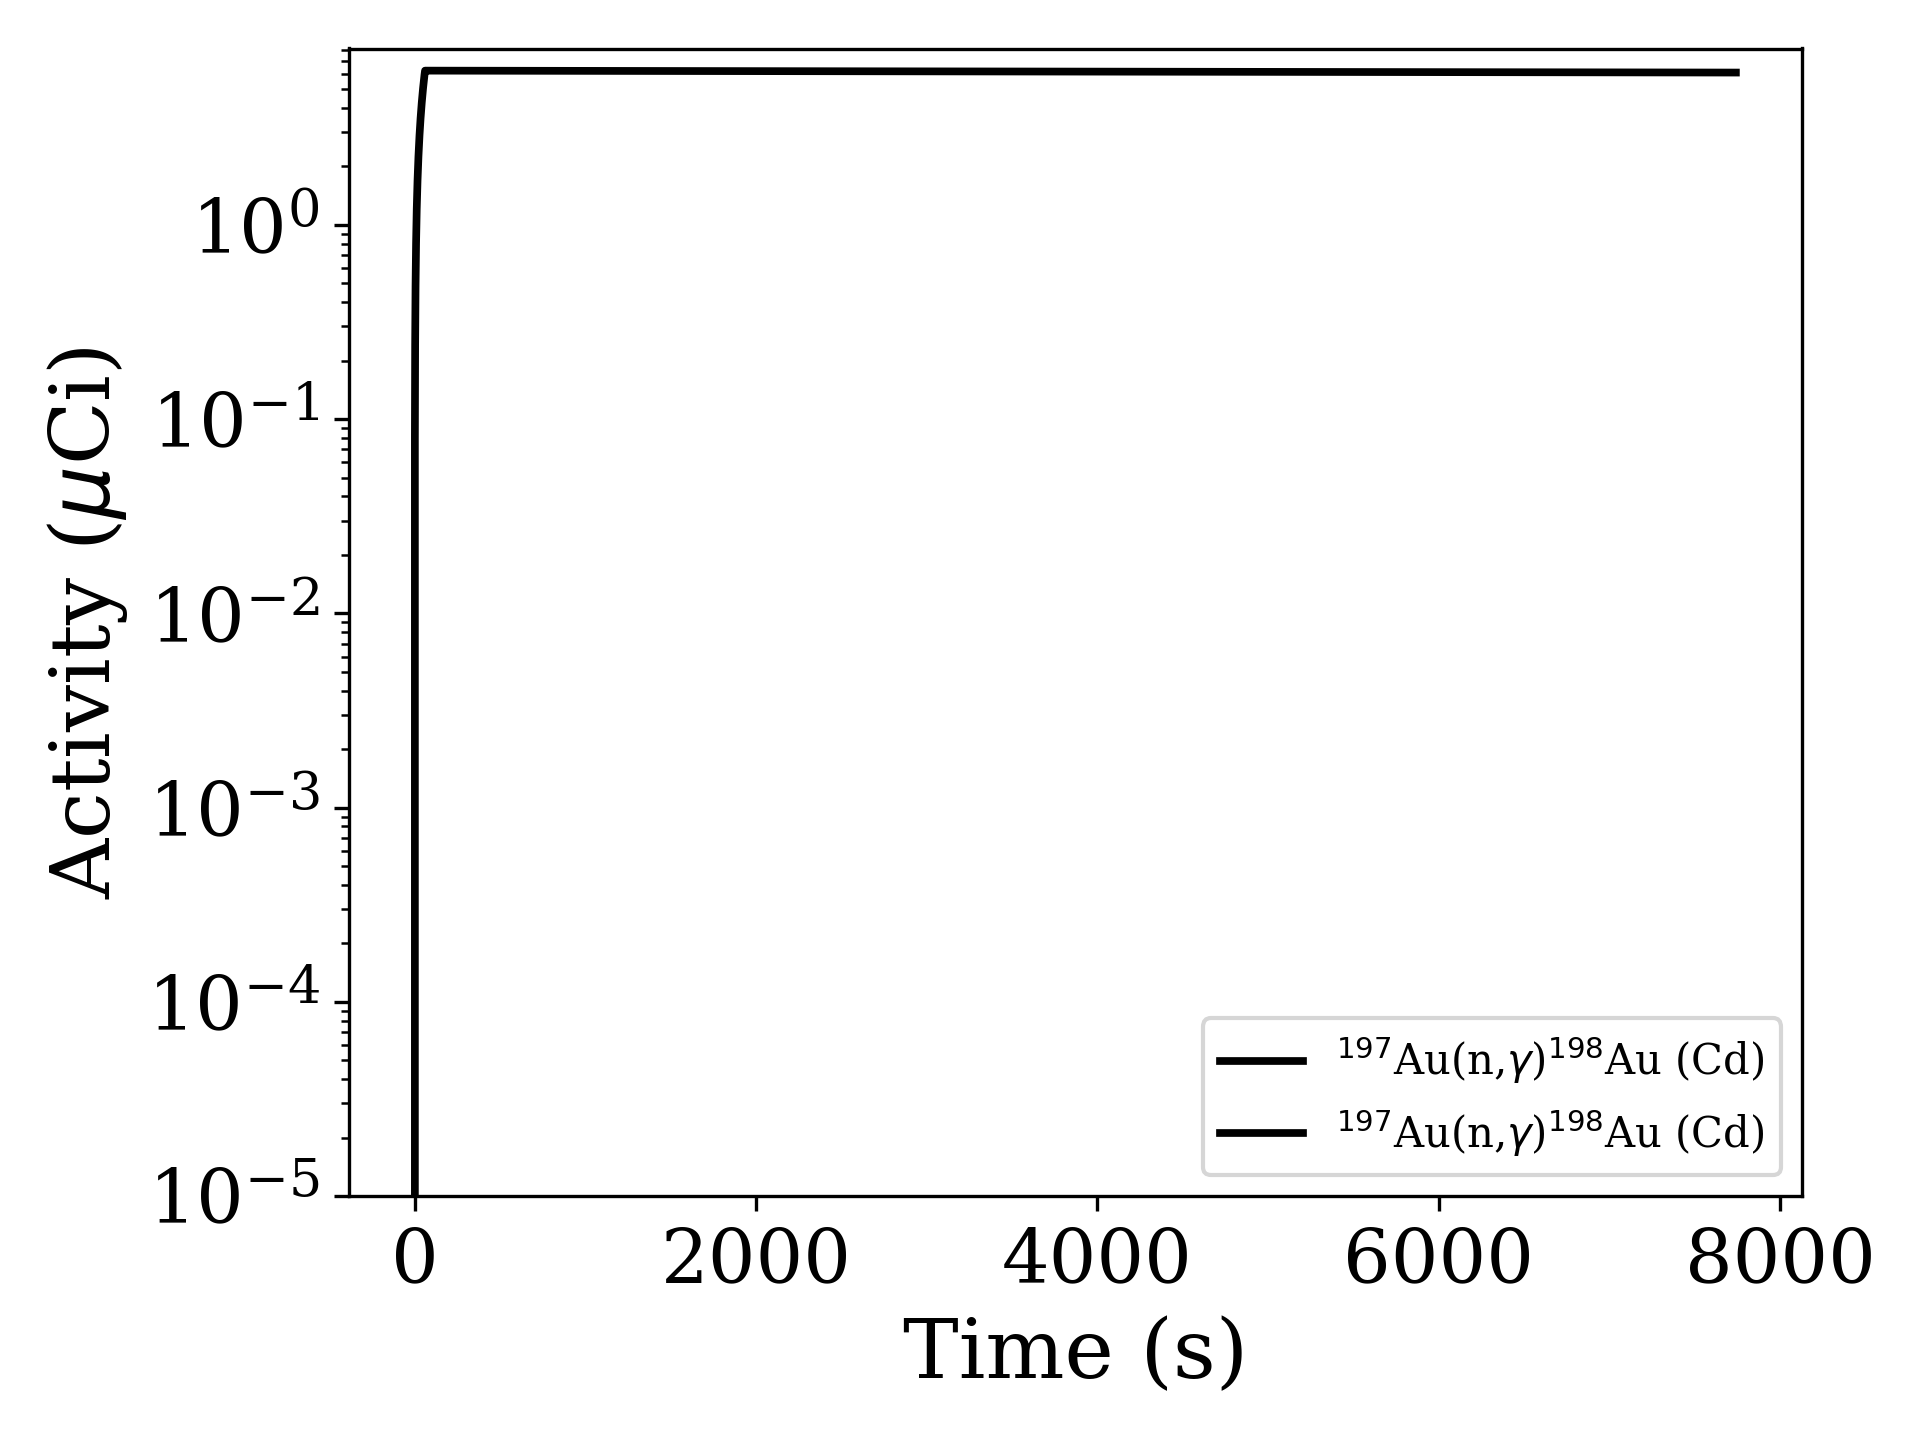
\includegraphics[width=.8\textwidth]{plot/Au-197(n,gamma)Au-198_Cd_wisconsin1} 

  \caption{Activity}
\end{subfigure}%
\begin{subfigure}{.5\textwidth}
  \centering
     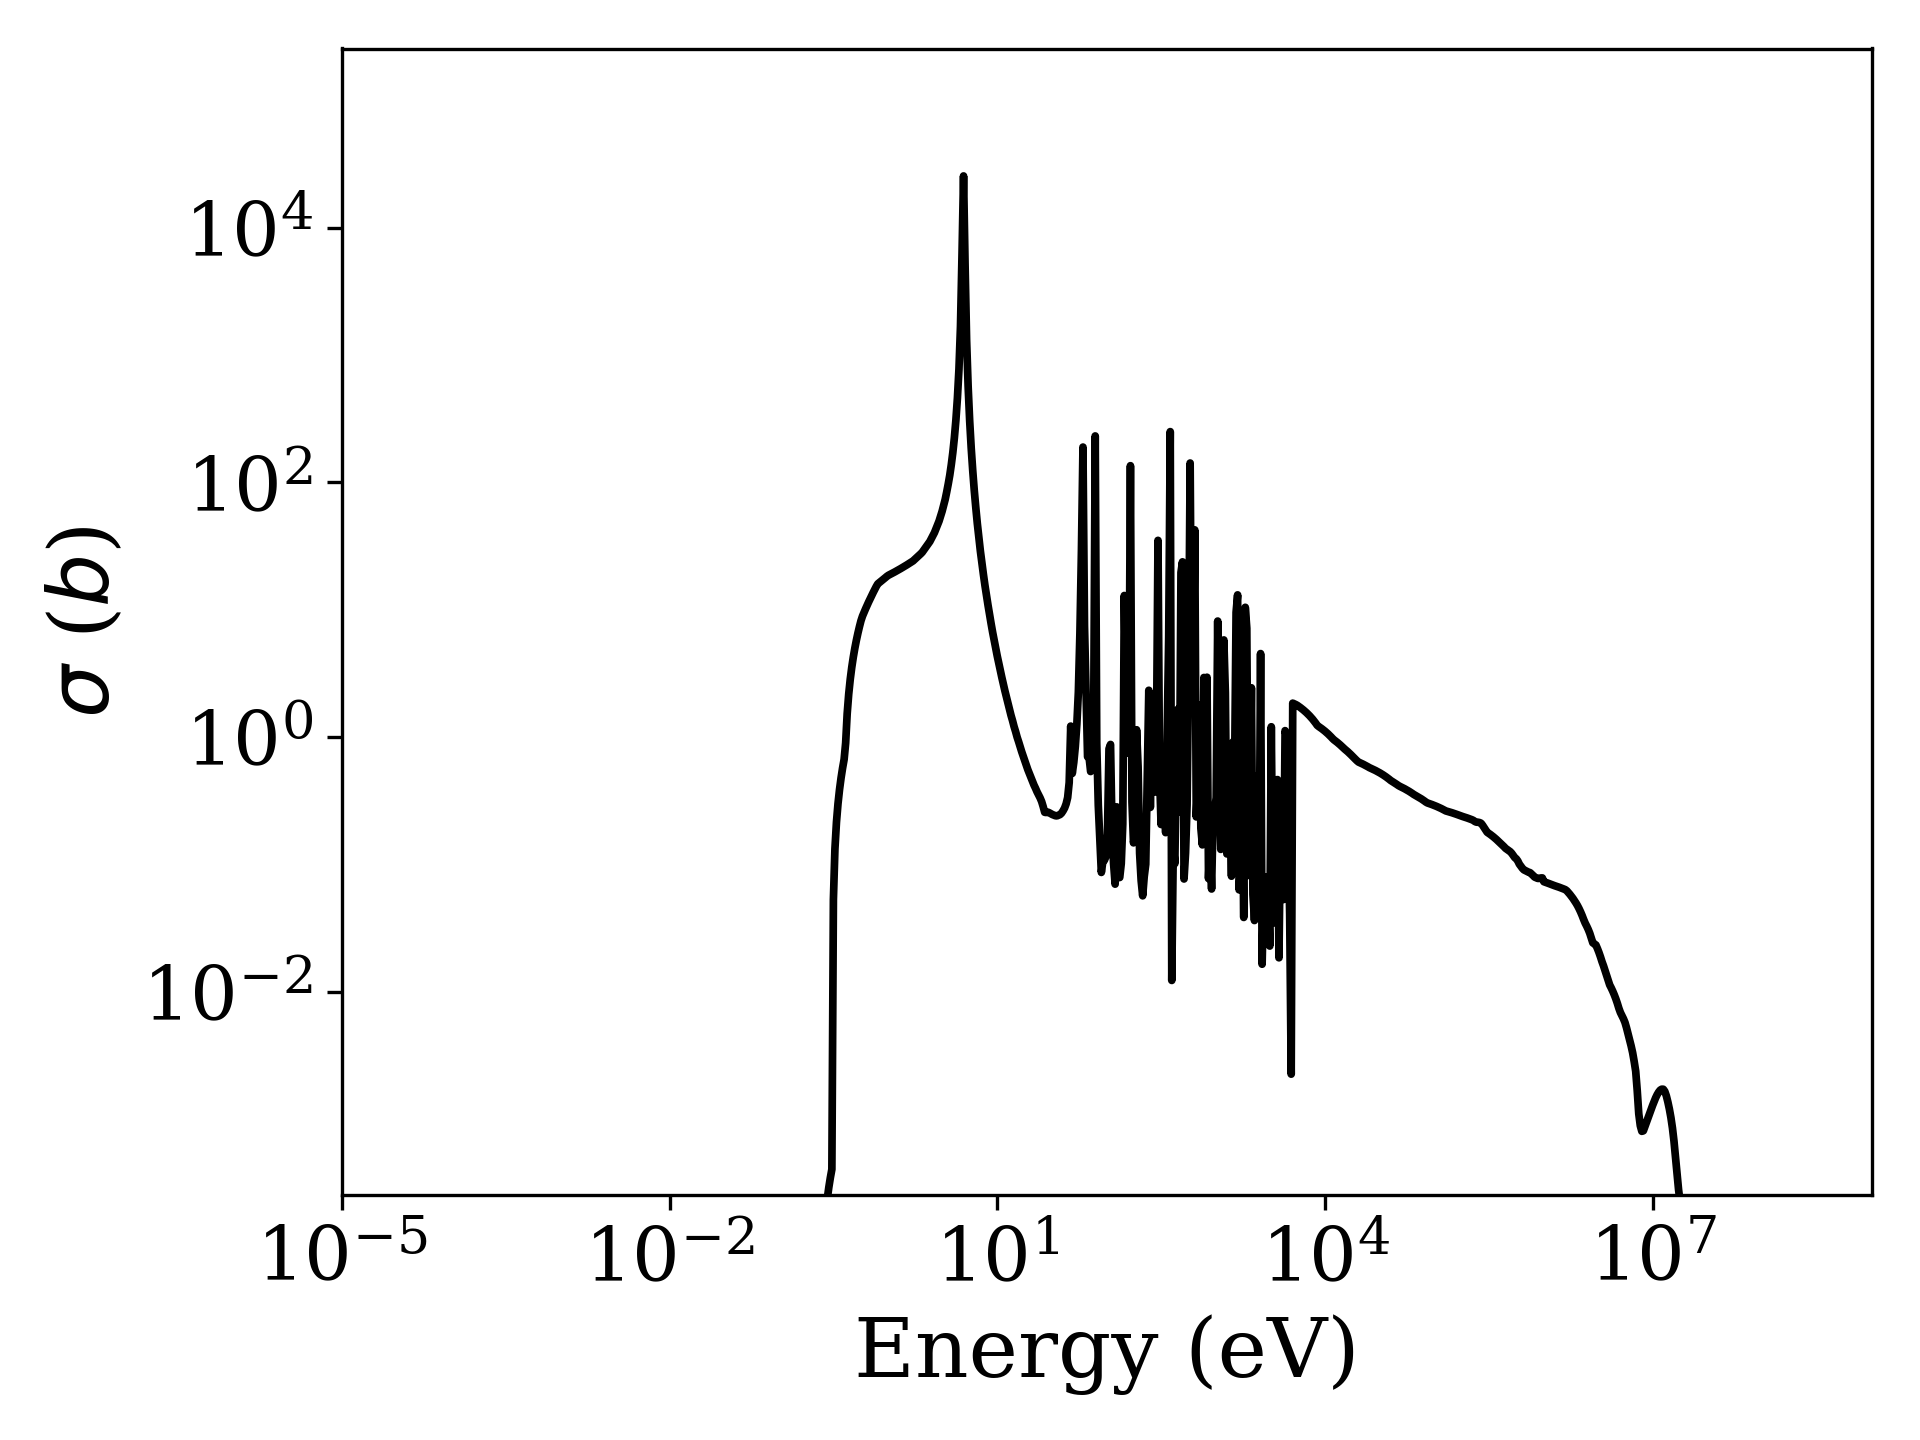
\includegraphics[width=.8\textwidth]{plot/Au-197(n,gamma)Au-198_Cd} 

  \caption{Cross Section}
\end{subfigure}
\end{figure}

\begin{table*}[h]
\centering
\begin{tabular}{ |c|c|c|c|c|c|c| }
 \hline
 Reaction & T$_{1/2}$ & ROI (eV) & Important Gammas (keV) \\
 \hline 
 $^{197}$Au(n,$\gamma$)$^{198}$Au (Cd) &  2.7 d & 3.99e+00, 5.99e+01 & 412(0.95) \\ 
\hline
\end{tabular}
\end{table*}
